%!TEX root = main.tex
\subsection{Figures for Dynamic Panel Simulation}
In this section we present figures to complement Table \ref{tab:Dpanel_RMSE} from Section \ref{sec:Dpanel_sim_SR}.
Figure \ref{fig:best} colors each region of the parameter space according to which of the estimators of $\theta$ -- $\text{LP}$, $\text{LS}$, $\text{P}$ or $\text{S}$ -- yields the lowest finite-sample RMSE.
The saturation of a color indicates the relative difference in RMSE of the lowest RMSE estimator at that point measured against the \emph{second lowest} RMSE estimator.
Darker indicates a larger advantage for the first-best estimator while lighter values indicate a smaller advantage. 
Figure \ref{fig:GFIC_rel_LP} depicts the relative different between the RMSE of the GFIC and that of the true specification, LP, expressed in percentage points.
Red indicates that the GFIC has the lower RMSE, blue that LP has the lower RMSE, and white that the RMSE values are the same. 
Darker colors indicate a larger difference.
Figure \ref{fig:RMSE_rel_oracle} compares the RMSE of the GFIC to that of the oracle procedure that uses whichever fixed specification -- LP, LS, P, or S -- yields the lowest finite sample MSE at a give point in the parameter space.
As in Figure \ref{fig:GFIC_rel_LP}, the comparison is one of relative RMSE in percentage points.
But, as the GFIC can by definition can never have a lower finite-sample MSE than the oracle estimator, the color scale used in this figure is different.
The remaining figures in this section compare the RMSE of the GFIC to that of the other selection procedures: GMM-AIC, GMM-BIC, etc.


%%%%%%%%%%%%%%%%%%%%%%%%%%%%%%%%%%%%%%%%
\begin{figure}[htbp]
\centering
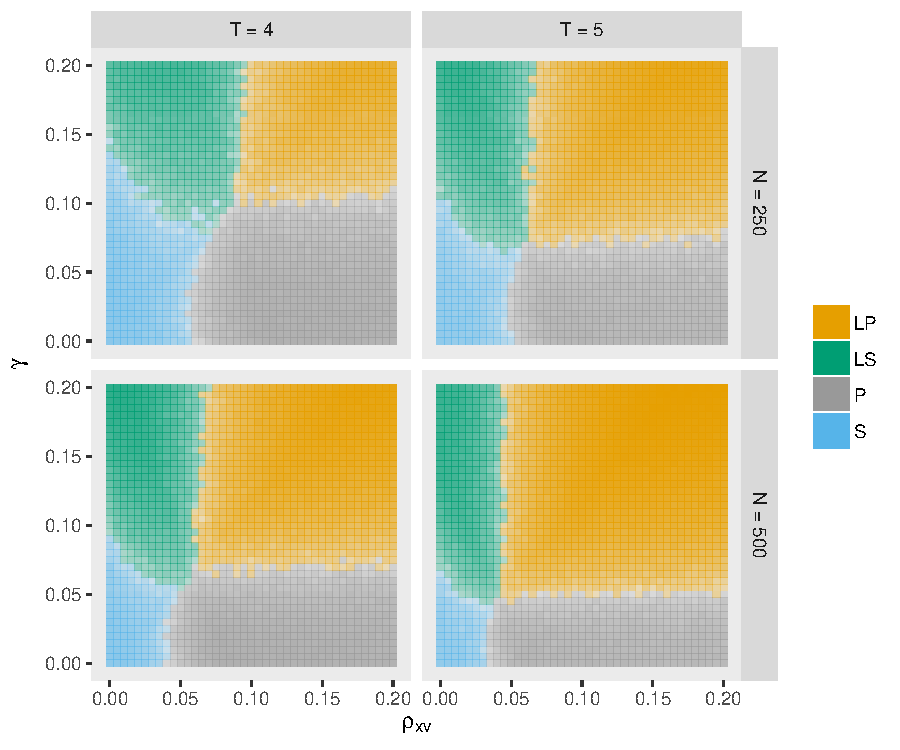
\includegraphics[scale = 0.8]{./simulations/DynamicPanel/results/Dpanel_oracle}
\caption{Minimum RMSE specification at each combination of parameter values for the simulation experiment from Section \ref{sec:Dpanel_sim_SR}. Color saturation at a given grid point indicates RMSE relative to second best specification.}
\label{fig:best}
\end{figure}
%%%%%%%%%%%%%%%%%%%%%%%%%%%%%%%%%%%%%%%%
\begin{figure}
\centering
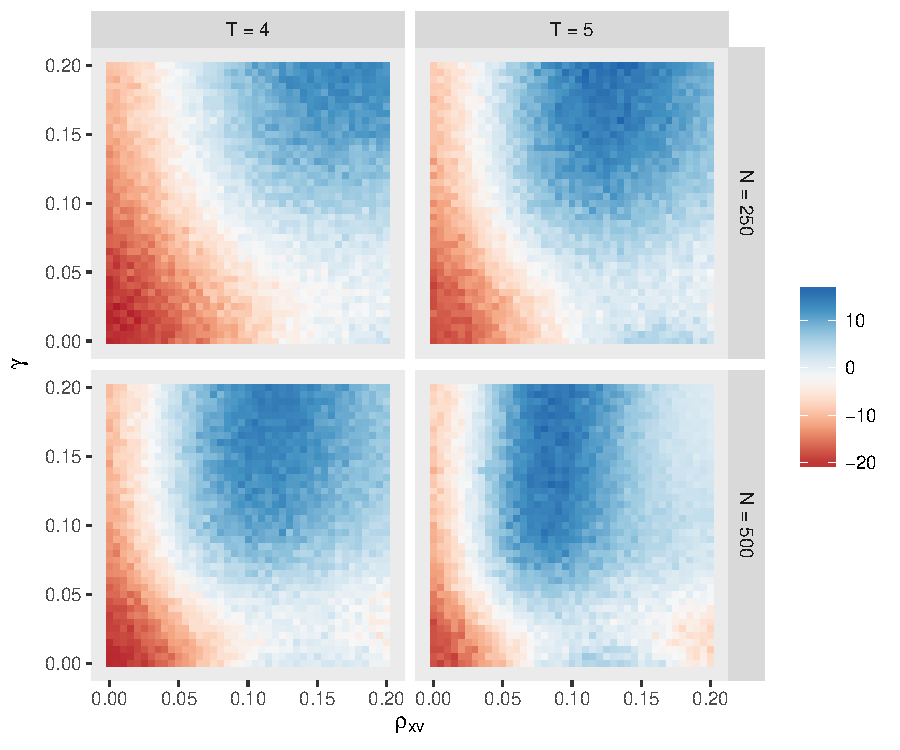
\includegraphics[scale = 0.8]{./simulations/DynamicPanel/results/Dpanel_GFIC_RMSE_rel_LP}
\caption{RMSE of the post-GFIC estimator relative to that of the true specification ($\text{LP}$) in the dynamic panel simulation experiment from Section \ref{sec:Dpanel_sim_SR}.}
\label{fig:GFIC_rel_LP}
\end{figure}
%%%%%%%%%%%%%%%%%%%%%%%%%%%%%%%%%%%%%%%%
\begin{figure}
\centering
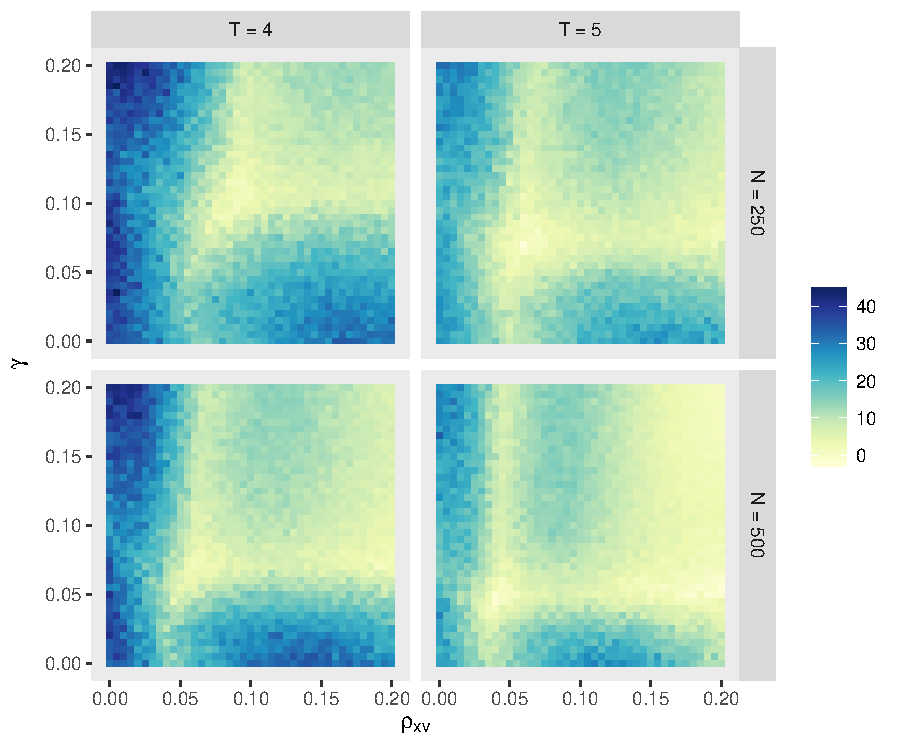
\includegraphics[scale = 0.8]{./simulations/DynamicPanel/results/Dpanel_GFIC_RMSE_rel_oracle}
\caption{RMSE of GFIC relative to Oracle Estimator in the Simulation from Section \ref{sec:Dpanel_sim_SR}}
\label{fig:RMSE_rel_oracle}
\end{figure}
%%%%%%%%%%%%%%%%%%%%%%%%%%%%%%%%%%%%%%%%
\begin{figure}
\centering
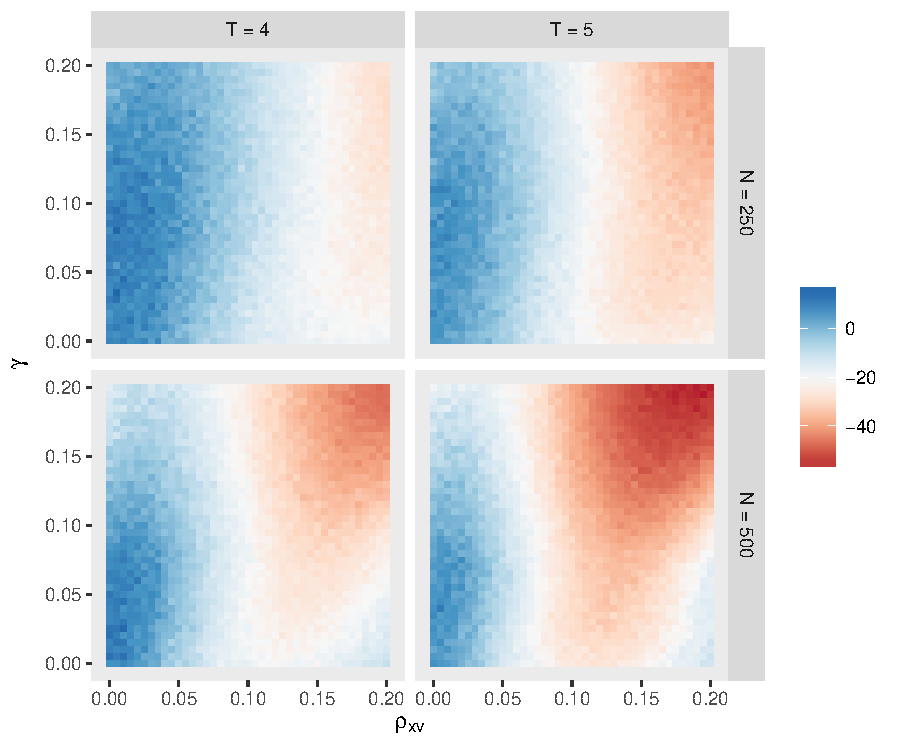
\includegraphics[scale = 0.8]{./simulations/DynamicPanel/results/Dpanel_GFIC_RMSE_rel_AIC}
\caption{RMSE of GFIC relative to GMM-AIC in the Simulation from Section \ref{sec:Dpanel_sim_SR}}
\end{figure}
%%%%%%%%%%%%%%%%%%%%%%%%%%%%%%%%%%%%%%%%
\begin{figure}
\centering
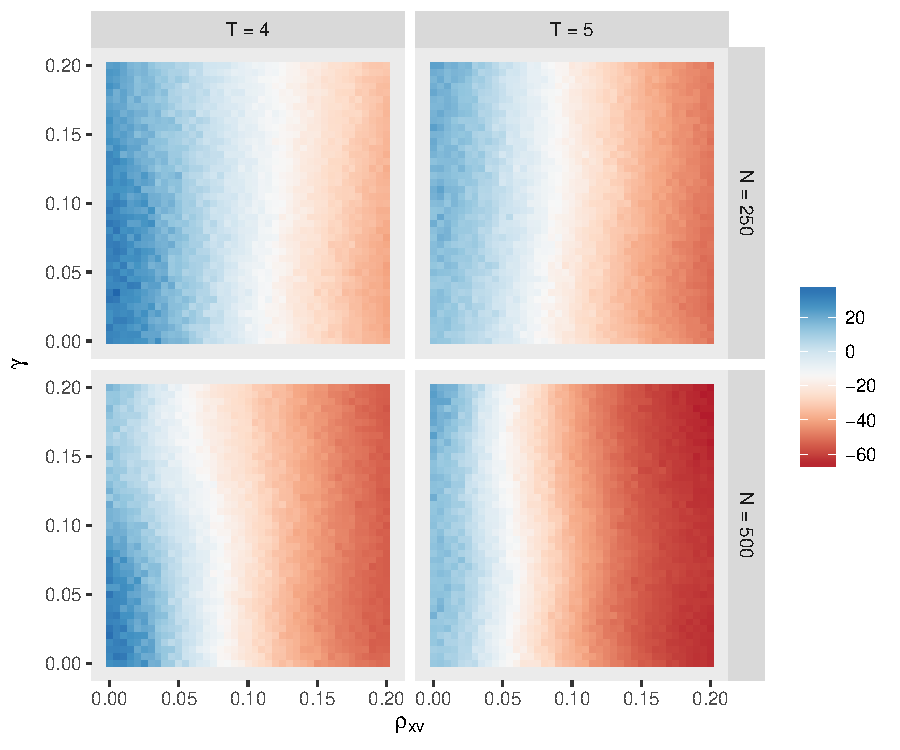
\includegraphics[scale = 0.8]{./simulations/DynamicPanel/results/Dpanel_GFIC_RMSE_rel_BIC}
\caption{RMSE of GFIC relative to GMM-BIC in the Simulation from Section \ref{sec:Dpanel_sim_SR}}
\end{figure}
%%%%%%%%%%%%%%%%%%%%%%%%%%%%%%%%%%%%%%%%
\begin{figure}
\centering
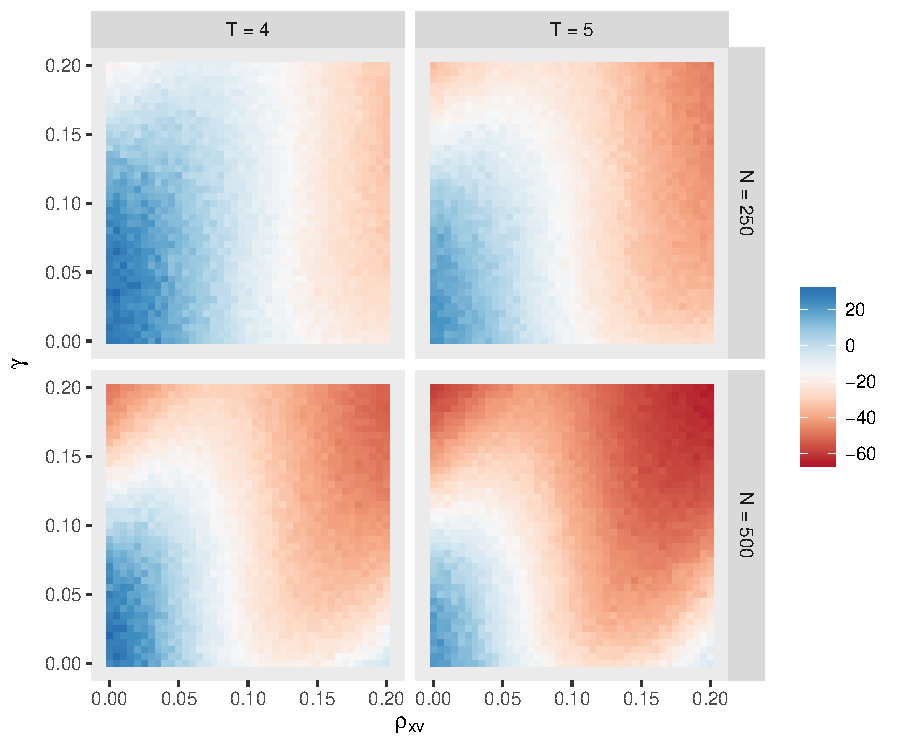
\includegraphics[scale = 0.8]{./simulations/DynamicPanel/results/Dpanel_GFIC_RMSE_rel_J5}
\caption{RMSE of GFIC relative to 5\% Downward J-test in the Simulation from Section \ref{sec:Dpanel_sim_SR}}
\end{figure}
%%%%%%%%%%%%%%%%%%%%%%%%%%%%%%%%%%%%%%%%
\begin{figure}
\centering
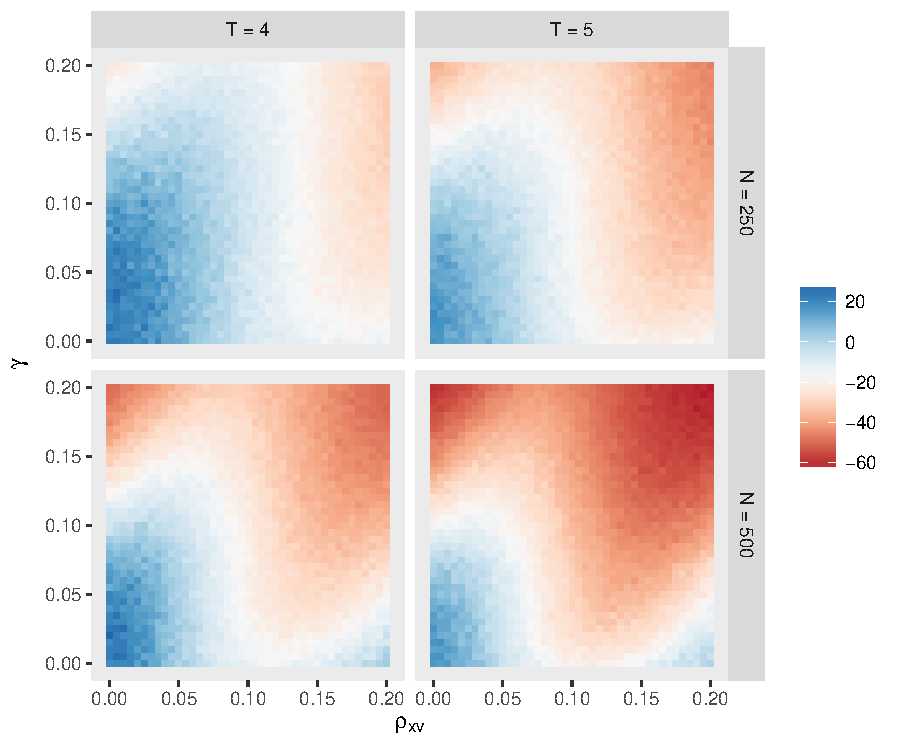
\includegraphics[scale = 0.8]{./simulations/DynamicPanel/results/Dpanel_GFIC_RMSE_rel_J10}
\caption{RMSE of GFIC relative to 10\% Downward J-test in the Simulation from Section \ref{sec:Dpanel_sim_SR}}
\end{figure}

%%%%%%%%%%%%%%%%%%%%%%%%%%%%%%%%%%%%%%%%
\begin{figure}
\centering
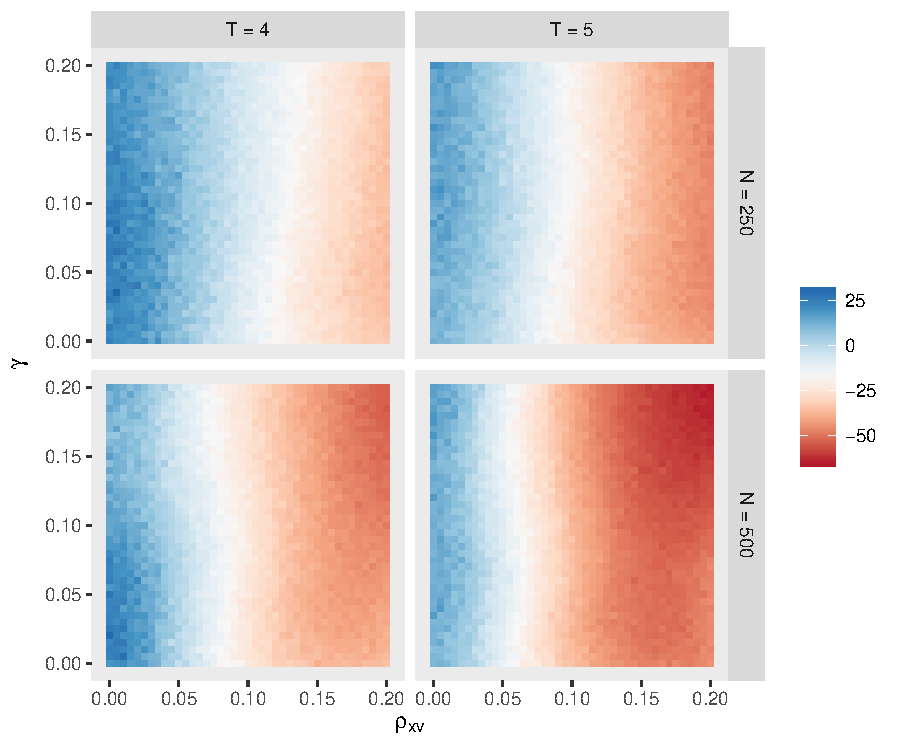
\includegraphics[scale = 0.8]{./simulations/DynamicPanel/results/Dpanel_GFIC_RMSE_rel_HQ}
\caption{RMSE of GFIC relative to GMM-HQ in the Simulation from Section \ref{sec:Dpanel_sim_SR}}
\end{figure}

%%%%%%%%%%%%%%%%%%%%%%%%%%%%%%%%%%%%%%%%
